% Báo cáo tiến độ, build riêng với báo cáo chính nhưng dùng chung config/, figures/, references.bib, latexmkrc.
%   cd report && latexmk tien-do.tex
% Kết quả: build/tien-do.pdf. Nhóm, GVHD, danh sách thành viên: chỉ sửa ở config/metadata.tex.
\documentclass[12pt,a4paper]{report}

% Preamble dùng chung. Biên dịch bằng XeLaTeX (xem latexmkrc).

% --- Ngôn ngữ và phông chữ (Unicode, không cần hack cho tiếng Việt) ---
\usepackage{fontspec}
\usepackage[vietnamese]{babel}
% Chọn font đầu tiên có trên máy: Times New Roman (msttcore-fonts) → Liberation (cùng kích thước,
% có sẵn trên đa số Linux) → TeX Gyre (có trong TeX Live đầy đủ / Overleaf, nạp theo tên file)
% → Latin Modern (mặc định của fontspec, luôn có). Font thực sự được dùng in ra log: tìm "Font chính:".
\newcommand{\chonfont}[4]{% #1 lệnh \set...font, #2 font ưu tiên, #3 font dự phòng, #4 tên file TeX Gyre
  \IfFontExistsTF{#2}{#1{#2}\typeout{Font chính: #2}}{%
    \IfFontExistsTF{#3}{#1{#3}\typeout{Font chính: #3 (thiếu #2)}}{%
      \IfFontExistsTF{#4-regular.otf}{%
        #1{#4}[Extension=.otf, UprightFont=*-regular, BoldFont=*-bold,
               ItalicFont=*-italic, BoldItalicFont=*-bolditalic]%
        \typeout{Font chính: #4 (thiếu #2 và #3)}}{%
        \typeout{Font chính: Latin Modern (thiếu #2, #3, #4)}}}}}
\chonfont{\setmainfont}{Times New Roman}{Liberation Serif}{texgyretermes}
\chonfont{\setsansfont}{Arial}{Liberation Sans}{texgyreheros}
\chonfont{\setmonofont}{Courier New}{Liberation Mono}{texgyrecursor}

% --- Cỡ chữ cố định theo bảng quy ước báo cáo/luận văn ---
% Thân bài 13pt · Mục lớn (section) 14pt · Mục con (subsection) 13pt đậm
% · Chú thích/footnote 10-12pt. Chương và header/listing đặt trực tiếp
% bằng \fontsize tại nơi dùng (xem macros.tex).
\makeatletter
\renewcommand\normalsize{\@setfontsize\normalsize{13}{15.6}} % thân bài: 13pt
\renewcommand\small{\@setfontsize\small{12}{14.4}}           % chú thích bảng/hình: 12pt
\renewcommand\footnotesize{\@setfontsize\footnotesize{10}{12}} % footnote: 10pt
\renewcommand\large{\@setfontsize\large{13}{15.6}}           % tiêu đề mục con (subsection): 13pt
\renewcommand\Large{\@setfontsize\Large{14}{16.8}}           % tiêu đề mục lớn (section): 14pt
\makeatother
\linespread{1.5}  % giãn dòng 1.5 (chuẩn báo cáo/luận văn)
\setlength{\parindent}{1cm}
\setlength{\parskip}{3pt}

% --- Bố cục: lề trái rộng hơn để đóng gáy ---
\usepackage[a4paper, left=3cm, right=2cm, top=2.5cm, bottom=2.5cm,
            headheight=40pt, headsep=1.0cm]{geometry}
\usepackage{fancyhdr}

% --- Toán, bảng, hình ---
\usepackage{amsmath}
\usepackage{amsthm}     % môi trường định lý / định nghĩa (khai báo ở macros.tex)
\usepackage{unicode-math}
\setmathfont{Latin Modern Math}  % font toán OpenType, chạy mọi cỡ chữ
\usepackage{booktabs, array, tabularx}
\usepackage{graphicx, float, caption}
\usepackage{subcaption}  % nhiều hình con trong một figure
\graphicspath{{figures/}} % \includegraphics tìm ảnh trong figures/
\captionsetup{font=small} % chú thích bảng/hình: 12pt (dùng cỡ \small đã đặt lại ở trên)
\usepackage{xcolor}
\usepackage{colortbl}    % tô màu hàng / ô của bảng
\usepackage{longtable}   % bảng dài tự ngắt trang
\usepackage{siunitx}     % số và đơn vị: \num{}, \SI{}{}, cột S căn theo dấu thập phân
\sisetup{output-decimal-marker={,}, group-separator={.}, group-minimum-digits=4}
\usepackage{algorithm, algorithmic} % khung thuật toán + mã giả
\usepackage{enumerate}
\usepackage[framemethod=tikz]{mdframed}
\usepackage{tikz}
\usetikzlibrary{arrows.meta, positioning}

% --- Mã nguồn ---
\usepackage{listings}

% --- Trích dẫn ---
%% Ghi chú: biblatex khuyến nghị csquotes, nhưng máy chạy lại không cài gói này;
%% thiếu nó chỉ sinh cảnh báo, không ảnh hưởng nội dung.
\usepackage[backend=biber, style=numeric, sorting=none]{biblatex}
\addbibresource{references.bib}
% biblatex không hỗ trợ tiếng Việt: ánh xạ sang tiếng Anh để các chuỗi
% "In:", "et al.", "and" hiện đúng thay vì rơi vào định nghĩa dự phòng hỏng.
\DeclareLanguageMapping{vietnamese}{english}

% --- Siêu liên kết (nạp sau cùng) ---
\usepackage{hyperref}

% Thông tin đề tài: chỉ sửa ở đây, trang bìa và tiêu đề PDF tự cập nhật.
\newcommand{\TenTruong}{Trường Đại học Sài Gòn}
\newcommand{\TenKhoa}{Khoa Công nghệ Thông tin}
\newcommand{\TenMonHoc}{Trí tuệ nhân tạo nâng cao}
\newcommand{\TenDeTai}{Xây dựng và đánh giá Game AI đa cấp độ cho Caro 11×11}
\newcommand{\TenNhom}{Nhóm 13}
\newcommand{\LinkRepo}{https://github.com/SGU-ML25/CaroGame}
\newcommand{\LoaiBaoCao}{Báo cáo đồ án cuối kỳ}
\newcommand{\CommitNop}{chưa chốt}

% Tên file PDF xuất ra cạnh main.tex sau mỗi lần build (không gồm đuôi .pdf; để trống {} thì không xuất).
% Không dùng lệnh LaTeX ở đây, chỉ chữ thường; latexmkrc đọc thẳng dòng này.
\newcommand{\TenFilePDF}{Nhóm 13 - Caro 11x11 - TTNTNC}
\newcommand{\TenFilePDFProposal}{Nhóm 13 - Caro 11x11 - Proposal}
\newcommand{\TenFilePDFDayDu}{Nhóm 13 - Caro 11x11 - Bao cao day du}

% Bản nháp / bản nộp. Nháp: dấu mờ "BẢN NHÁP", hiện \goiy và \chualam.
% Nộp (\BanNoptrue): không dấu mờ; còn sót \goiy hoặc \chualam thì build báo lỗi.
\newif\ifBanNop
\BanNopfalse

\newcommand{\GVHD}{TS. Đỗ Như Tài}
\newcommand{\ThoiGian}{TP. Hồ Chí Minh, tháng 11/2026}

% Danh sách sinh viên: mỗi dòng "& Họ tên & MSSV \\" (cột đầu để trống)
\newcommand{\DanhSachSV}{%
  & Huỳnh Thanh Tiến & 3123410374 \\
  & Đặng Ngọc Như Ý  & 3123410438 \\
  & Võ Thị Như Ý     & 3123410439 \\
}

% Macro, màu sắc, thiết lập listings / hyperref / header.

\definecolor{dkgreen}{rgb}{0,0.6,0}
\definecolor{gray}{rgb}{0.5,0.5,0.5}
\definecolor{mauve}{rgb}{0.58,0,0.82}

\hypersetup{
  urlcolor=blue, linkcolor=black, citecolor=black, colorlinks=true,
  pdftitle={\TenDeTai}, pdfauthor={\TenKhoa, \TenTruong},
}

% --- Mã nguồn: listings chỉ dựng bảng ký tự cho mã 0--255. Chữ tiếng Việt có dấu (mã > 255) bị in
% ngay trong khi chữ ASCII còn nằm trong bộ đệm, làm đảo thứ tự ("hoặc" thành "ặhoc"). Hook dưới đây
% đăng ký các chữ đó là chữ cái của listings, giống cách listings tự làm với a--z. ---
\makeatletter
\def\lst@VNletters{258,259,272,273,296,297,360,361,416,417,431,432,7840,7841,7842,7843,7844,7845,7846,7847,7848,7849,7850,7851,7852,7853,7854,7855,7856,7857,7858,7859,7860,7861,7862,7863,7864,7865,7866,7867,7868,7869,7870,7871,7872,7873,7874,7875,7876,7877,7878,7879,7880,7881,7882,7883,7884,7885,7886,7887,7888,7889,7890,7891,7892,7893,7894,7895,7896,7897,7898,7899,7900,7901,7902,7903,7904,7905,7906,7907,7908,7909,7910,7911,7912,7913,7914,7915,7916,7917,7918,7919,7920,7921,7922,7923,7924,7925,7926,7927,7928,7929,9472,9474,9492,9500}
\lst@AddToHook{SelectCharTable}{%
  \@for\lst@vn:=\lst@VNletters\do{%
    \catcode\lst@vn=\active
    \begingroup\lccode`\~=\lst@vn\relax\lccode`\/=\lst@vn\relax
    \lowercase{\endgroup\def~{\lst@ProcessLetter/}}}}
\makeatother

\lstset{
  frame=tb,
  language=Python,
  aboveskip=3mm,
  belowskip=3mm,
  showstringspaces=false,
  columns=flexible,
  basicstyle={\fontsize{10.5}{12.6}\selectfont\ttfamily}, % code/listing: 10.5pt
  numbers=left,
  numberstyle=\tiny\color{gray},
  keywordstyle=\color{blue},
  commentstyle=\color{dkgreen},
  stringstyle=\color{mauve},
  breaklines=true,
  breakatwhitespace=true,
  tabsize=3,
  numbersep=5pt,
  escapeinside={(*@}{@*)},
  captionpos=t
}

% --- Kiểu cho mã LaTeX (dùng trong tài liệu hướng dẫn): \begin{lstlisting}[style=latex] ---
\lstdefinestyle{latex}{language=[LaTeX]TeX, numbers=none, backgroundcolor=\color{gray!8},
  texcsstyle=*\color{blue}, moretexcs={includegraphics,subcaption,caption,label,ref,cite,toprule,midrule,bottomrule,
  multicolumn,rowcolor,cellcolor,num,SI,eqref,goiy,chualam,chuatrienkhai,lstinputlisting,url,href,textcite,
  autoref,cline,addplot,draw,node,STATE,IF,ELSE,ENDIF,FOR,ENDFOR,RETURN,REQUIRE,ENSURE,WHILE,ENDWHILE}}

% --- Định lý / định nghĩa / ví dụ (amsthm), đánh số theo chương ---
\theoremstyle{plain}
\newtheorem{dinhly}{Định lý}[chapter]
\theoremstyle{definition}
\newtheorem{dinhnghia}{Định nghĩa}[chapter]
\newtheorem{vidu}{Ví dụ}[chapter]
\theoremstyle{remark}
\newtheorem*{nhanxet}{Nhận xét}

% --- Tên tiếng Việt cho khung thuật toán ---
\floatname{algorithm}{Thuật toán}
\renewcommand{\algorithmicrequire}{\textbf{Đầu vào:}}
\renewcommand{\algorithmicensure}{\textbf{Đầu ra:}}

% --- Đánh số "Đoạn mã N.M" cho lstlisting, theo chương, giống Bảng/Hình ---
% (listings tự đặt lại số theo chương khi lớp tài liệu có \thechapter)
\renewcommand{\lstlistingname}{Đoạn mã}
\renewcommand{\lstlistlistingname}{Danh sách đoạn mã}

% --- Hộp ghi chú cho phần chưa triển khai ---
\newcommand{\chuatrienkhai}[1]{%
  \begin{mdframed}[backgroundcolor=yellow!15, linecolor=orange, linewidth=1pt]
    \textbf{Chưa triển khai.} #1
  \end{mdframed}}

% --- Ghi chú ngắn cho nội dung sẽ bổ sung ở các tuần sau ---
% --- Gợi ý nội dung cần viết trong sườn bài (xoá khi viết xong mục) ---
% Ở bản nộp (\BanNoptrue trong metadata.tex) cả hai báo lỗi để không nộp sót.
\ifBanNop
  \newcommand{\chualam}[1]{\PackageError{baocao}{Bản nộp còn \string\chualam{#1}}{Viết xong rồi xoá lệnh này.}}
  \newcommand{\goiy}[1]{\PackageError{baocao}{Bản nộp còn \string\goiy{#1}}{Viết xong mục rồi xoá lệnh này.}}
\else
  \newcommand{\chualam}[1]{\textit{(Chưa làm --- #1)}}
  \newcommand{\goiy}[1]{{\color{gray}\itshape [Cần viết: #1]}\par}
\fi

% --- Dấu mờ "BẢN NHÁP" trên mọi trang khi chưa bật \BanNoptrue ---
\AddToHook{shipout/background}{%
  \ifBanNop\else
    \put(0.5\paperwidth,-0.5\paperheight){\makebox(0,0){\rotatebox{45}{%
      \fontsize{90}{90}\selectfont\bfseries\color{gray!12}BẢN NHÁP}}}%
  \fi}

% --- Logo: bỏ qua êm nếu chưa có file figures/logoITSGU.png ---
\newcommand{\logo}[1]{\IfFileExists{figures/logoITSGU.png}%
  {
\includegraphics[#1]{figures/logoITSGU.png}}{}}

% --- Header / footer ---
\setlength{\headheight}{40pt}
\renewcommand{\headrule}{\vskip 2pt\hrule height 0.4pt\vskip 0pt}
\pagestyle{fancy}
\fancyhf{}
\fancyhead[L]{%
  \begin{tabular}{rl}
    \begin{picture}(25,15)(0,0)
      \put(0,-8){\logo{width=8mm,height=8mm}}
    \end{picture} &
    \begin{tabular}[c]{l}
      \normalfont\fontsize{11}{13}\selectfont \TenTruong \\ \TenKhoa % header: 11pt
    \end{tabular}
  \end{tabular}}
\fancyfoot[C]{\thepage}
\renewcommand{\headrulewidth}{0.4pt}
% Trang mở đầu chương dùng cùng kiểu header
\fancypagestyle{plain}{\pagestyle{fancy}}

\setcounter{secnumdepth}{3}
\setcounter{tocdepth}{2}

% --- Tiêu đề chương: căn giữa, in hoa, đậm, một dòng "CHƯƠNG N. TÊN" ---
\makeatletter
\def\@makechapterhead#1{%
  {\parindent\z@ \centering \normalfont\fontsize{17}{20}\selectfont\bfseries % tiêu đề chương: 17pt
   \MakeUppercase{\@chapapp\ \thechapter.\ #1}\par\nobreak
   \vskip 18\p@}}
\def\@makeschapterhead#1{%
  {\parindent\z@ \centering \normalfont\fontsize{17}{20}\selectfont\bfseries % tiêu đề chương: 17pt
   \MakeUppercase{#1}\par\nobreak
   \vskip 18\p@}}
\makeatother

% --- \texttt cho phép xuống dòng sau / _ . để tên file không tràn lề ---
\let\oldtexttt\texttt
\ExplSyntaxOn
\tl_new:N \l__tt_break_tl
\RenewDocumentCommand{\texttt}{m}
  {
    \tl_set:Nn \l__tt_break_tl {#1}
    \tl_replace_all:Nnn \l__tt_break_tl { \_ } { \_ \allowbreak }
    \tl_replace_all:Nnn \l__tt_break_tl { / } { / \allowbreak }
    \tl_replace_all:Nnn \l__tt_break_tl { . } { . \allowbreak }
    \tl_replace_all:Nnn \l__tt_break_tl { - } { - \allowbreak }
    \exp_args:NV \oldtexttt \l__tt_break_tl
  }
\ExplSyntaxOff
\emergencystretch=2em

% --- Từ khoá tiếng Việt cho mã giả (algorithmic) ---
\renewcommand{\algorithmicif}{\textbf{nếu}}
\renewcommand{\algorithmicthen}{\textbf{thì}}
\renewcommand{\algorithmicelse}{\textbf{ngược lại}}
\renewcommand{\algorithmicend}{\textbf{hết}}
\renewcommand{\algorithmicfor}{\textbf{với}}
\renewcommand{\algorithmicdo}{\textbf{làm}}
\renewcommand{\algorithmicwhile}{\textbf{trong khi}}
\renewcommand{\algorithmicreturn}{\textbf{trả về}}

% --- Tên lệnh LaTeX trong bảng / chú thích: \cmd{goiy\{...\}} → \goiy{...} ---
\newcommand{\cmd}[1]{\texttt{\textbackslash #1}}



% --- Điều chỉnh riêng: chữ nhỏ, lề hẹp, không chương, không dấu "BẢN NHÁP" (giống proposal.tex) ---
\RemoveFromHook{shipout/background}[top-level]
\geometry{left=2.2cm, right=2cm, top=2.4cm, bottom=2cm, headheight=40pt, headsep=0.5cm}
\setlength{\headwidth}{\textwidth}
\makeatletter
\renewcommand\normalsize{\@setfontsize\normalsize{12}{14.4}}
\renewcommand\small{\@setfontsize\small{10.5}{12.6}}
\def\@seccntformat#1{\csname the#1\endcsname.\quad}
\makeatother
\normalsize
\linespread{1.12}
\setlength{\parindent}{0pt}
\setlength{\parskip}{4pt}

\renewcommand{\thesection}{\arabic{section}}
\renewcommand{\thefigure}{\arabic{figure}}
\renewcommand{\thetable}{\arabic{table}}
\captionsetup{font={small,it}, labelfont={bf,up}}
\hypersetup{pdftitle={Báo cáo tiến độ: Game AI đa cấp độ, Caro 11×11 (\TenNhom)}}

\fancyfoot[C]{\small Báo cáo tiến độ -- Game AI Caro 11×11 -- Trang \thepage}

\usetikzlibrary{calc, fit, shapes.misc}
\definecolor{xanhdam}{HTML}{0B4A7C}
\definecolor{xanhnhat}{HTML}{E4EEF6}
\definecolor{luc}{HTML}{1B7F4B}
\definecolor{cam}{HTML}{B65C00}
\newenvironment{gon}{\begin{itemize}\setlength{\itemsep}{2pt}\setlength{\parskip}{0pt}}{\end{itemize}}

\begin{document}

% ============================== TIÊU ĐỀ ==============================
\begin{center}
  {\fontsize{17}{21}\selectfont\bfseries\color{xanhdam} BÁO CÁO TIẾN ĐỘ\par}
  \vspace{2pt}
  {\large\itshape \TenMonHoc\par}
  \vspace{6pt}
  {\bfseries \TenDeTai\par}
  \vspace{4pt}
  {\small \TenNhom\ -- GVHD: \GVHD\ -- Cập nhật ngày 15/11/2026\\ Mã nguồn: \url{\LinkRepo}\par}
\end{center}
\hrule\vspace{6pt}

% ============================== 1 ==============================
\section{TÓM TẮT}
Đề tài xây dựng tám cấp tác tử cho Caro 11×11 rồi so sánh chúng bằng thực nghiệm có kiểm soát. Báo cáo này tổng kết những gì đã làm được đến ngày 15/11/2026, các số liệu nhóm đã đo, những vấn đề đang gặp và kế hoạch cho phần còn lại.

\textbf{Những gì đã có.} Engine bitboard, bốn tác tử đầu (Random, luật, Alpha-Beta, MCTS), khung giải đấu có thống kê, giao diện web, hệ thống cấu hình và ghi log, cùng khoảng 200 kiểm thử tự động. Các thí nghiệm A1, A2, A3, A4 và A7 đã chạy và có số liệu. Cấp 6 (REINFORCE có baseline) đã viết xong và có kiểm thử trên nhánh \texttt{feat/l6-reinforce}, chưa merge.

\textbf{Những gì đang chậm.} Cấp 5 (học có giám sát) chưa huấn luyện được vì dữ liệu chuyên gia chưa sinh. Với cấu hình mặc định, sinh \num{20000} ván mất khoảng $11{,}8$ giờ trên máy của nhóm. Nhóm đã tìm ra điểm nghẽn ở hàm \texttt{scored\_moves} và thử nghiệm sơ bộ cho thấy cắt tỉa ở gốc có thể giảm còn khoảng $3{,}5$ giờ mà không đổi kết quả top-3.

\textbf{Những gì chưa làm.} Huấn luyện cấp 5 và 6, cấp 7 (PUCT) và cấp 8 (vòng lặp AlphaZero), giải đấu chính ở hai chế độ ngân sách, các thí nghiệm A5, A5b, A6, E3, và phần phân tích tổng hợp.

\begin{table}[h]
  \centering\small
  \begin{tabular}{@{}llp{7.6cm}@{}}
    \toprule
    Hạng mục & Trạng thái & Ghi chú \\
    \midrule
    Engine bitboard & Xong & Kiểm tra thắng, ứng viên, Zobrist, đối xứng; có kiểm thử \\
    Cấp 1 Random, Cấp 2 luật & Xong & Cấp 2 gồm các luật P1--P7 \\
    Cấp 3 Alpha-Beta & Xong & Cắt tỉa, sắp xếp nước, bảng chuyển vị, nước bắt buộc \\
    Cấp 4 MCTS (UCT) & Xong & Rollout ngẫu nhiên và nhẹ; tuỳ chọn xử lý chiến thuật ở gốc \\
    Khung giải đấu, thống kê & Xong & Vòng tròn, khai cuộc đổi màu, khoảng Wilson, Elo \\
    Giao diện web & Xong & Người--máy, máy--máy, xem lại ván \\
    Cấp 5 học có giám sát & Đang làm & Code có; chờ dữ liệu chuyên gia \\
    Cấp 6 REINFORCE & Code xong & Nhánh \texttt{feat/l6-reinforce}, chưa chạy thật \\
    Cấp 7 PUCT, cấp 8 AlphaZero & Chưa làm & Phụ thuộc cấp 5 \\
    Thí nghiệm A1, A2, A3, A4, A7 & Có số liệu & Một số cần đo lại (mục~\ref{sec:thucnghiem}) \\
    Thí nghiệm A5, A5b, A6, E3 & Chưa làm & Phụ thuộc mô hình học được \\
    \bottomrule
  \end{tabular}
  \caption{Trạng thái các hạng mục tại ngày 15/11/2026.}
\end{table}

% ============================== 2 ==============================
\section{DÒNG THỜI GIAN CÔNG VIỆC}
Dự án có 43 commit không tính merge, bắt đầu từ 18/10/2026. Các mốc chính, theo các pull request đã merge vào \texttt{main}:

\begin{table}[h]
  \centering\small
  \begin{tabularx}{\textwidth}{@{}l l X@{}}
    \toprule
    Ngày & Pull request & Nội dung \\
    \midrule
    18/10 & --- & Khởi tạo repo, tài liệu hướng dẫn, cấu hình, engine, kiểm thử và notebook thử engine \\
    26--28/10 & \#27, \#28 & Cấp 2 (luật), cấp 3 Alpha-Beta, các nhánh \texttt{tv2-nhu-y} \\
    28/10 & \#29 & Khung báo cáo LaTeX \\
    04/11 & \#30, \#31 & Thí nghiệm A1, A2 (nhánh \texttt{tv2-nhu-y-a1a2}); giao diện web \\
    07/11 & \#32, \#33 & Khung giải đấu (\texttt{tv4-arena}) và thống kê (\texttt{tv4-stats}) \\
    13/11 & \#34, \#35 & Cấp 4 MCTS; mạng nơ-ron và dataset (\texttt{tv4-nn}) \\
    15/11 & \#36, \#37 & Thí nghiệm A3, A4 (có notebook); sinh dữ liệu và huấn luyện có giám sát (\texttt{tv4-sl-training}) \\
    15/11 & --- & Cấp 6 REINFORCE: commit \texttt{af8312f} trên \texttt{feat/l6-reinforce}, chưa tạo PR \\
    \bottomrule
  \end{tabularx}
  \caption{Các mốc chính của dự án.}
\end{table}

% ============================== 3 ==============================
\section{HẠ TẦNG VÀ CÁC TÁC TỬ ĐÃ HOÀN THÀNH}

\subsection{Engine bitboard}
Mỗi bên được biểu diễn bằng một số nguyên 121 bit (bàn $11\times11$, bố cục \texttt{stride11}, bit $i$ là ô $i$), nên cả bàn cờ vừa một số nguyên 128 bit. Luật là ``từ 5 quân liên tiếp là thắng, không luật chặn hai đầu''. Các thao tác cốt lõi đều là phép dịch bit và phép toán logic:
\begin{gon}
  \item \textbf{Kiểm tra thắng} bằng ba phép dịch bit cho mỗi hướng, dùng mặt nạ để quân không tràn qua biên bàn.
  \item \textbf{Sinh nước ứng viên} bằng phép giãn nở các quân đã có với bán kính 1 hoặc 2, thay vì xét cả 121 ô.
  \item \textbf{Đếm quân trong mọi cửa sổ 5 ô} và \textbf{tìm ô thắng ngay}, làm nền tảng cho hàm đánh giá và các luật chiến thuật.
  \item \textbf{Băm Zobrist} cho bảng chuyển vị, và \textbf{8 phép đối xứng} của bàn vuông (4 phép quay, mỗi phép có thêm bản đối xứng gương), dùng cho tăng cường dữ liệu và loại trùng lặp.
\end{gon}
Giao diện trò chơi thống nhất (\texttt{CaroGame}) cung cấp \texttt{step}, \texttt{legal\_actions}, \texttt{is\_terminal}, \texttt{winner}, \texttt{key} và \texttt{history}, và mọi tác tử chỉ giao tiếp với trò chơi qua giao diện này. Engine được kiểm thử bằng 33 kiểm thử bitboard, 20 kiểm thử game, 4 kiểm thử đối xứng và một bản cài đặt ngây thơ (\texttt{tests/naive.py}) để đối chiếu kết quả.

\subsection{Giao diện tác tử}
Mọi tác tử kế thừa \texttt{BaseAgent} với phương thức \texttt{select\_action(game, limits)}. \texttt{Limits} gói ngân sách của một nước đi: thời gian (ms), độ sâu tối đa hoặc số mô phỏng tối đa, kèm hàm tính hạn chót. Nhờ vậy giải đấu áp dụng cùng một cơ chế ngân sách cho mọi cấp và \texttt{make\_agent} dựng tác tử từ một file cấu hình YAML.

\subsection{Cấp 1 và cấp 2}
Cấp 1 chọn ngẫu nhiên trong các ô hợp lệ, dùng làm đường cơ sở dưới cùng. Cấp 2 là tác tử luật gồm bảy luật ưu tiên P1 đến P7, mỗi luật tính bằng các hàm bitboard có sẵn, chỉ nhìn trước đúng một nước (không tìm kiếm cây). Danh sách luật bật được cấu hình qua tham số \texttt{priorities}; có 20 kiểm thử, gồm các ca xung đột giữa luật (P3--P4, P4--P5). Smoke test cho thấy cấp 2 thắng Random 100\%, và cấp 3 thắng cấp 2 với khoảng Wilson $[53{,}1\%;\ 88{,}8\%]$ không chứa $50\%$ (mẫu nhỏ, chỉ để kiểm tra pipeline).

\subsection{Cấp 3: Negamax Alpha-Beta}
Cài đặt đầy đủ các kỹ thuật chuẩn: negamax, cắt tỉa alpha-beta, đào sâu dần (iterative deepening), bảng chuyển vị Zobrist (mặc định 64 MB), sắp xếp nước, và xử lý nước bắt buộc (thắng ngay, chặn tứ). Tập nước ứng viên là phép giãn nở bán kính 2 quanh các quân. Mỗi kỹ thuật bật tắt được bằng tham số cấu hình, nhờ đó thí nghiệm A1, A2 và A7 chỉ cần đổi cấu hình. Hàm đánh giá dùng các cửa sổ 5 ô với trọng số cho cả tấn công và phòng thủ; tham số \texttt{eval\_weights} cho phép bỏ phần phòng thủ để làm thí nghiệm A7.

Ngoài \texttt{select\_action}, tác tử có hàm \texttt{scored\_moves(game, limits, top\_k)} trả về top-$k$ nước kèm điểm, dùng để sinh dữ liệu chuyên gia cho cấp 5. Hàm này là nguồn gốc của vấn đề thời gian ở mục~\ref{sec:thoigian}.

\subsection{Cấp 4: MCTS với UCT}
Cài đặt chọn nút bằng công thức UCT với hằng số thăm dò $c = 1{,}4$, hai kiểu rollout (\texttt{random} và \texttt{light}), bán kính ứng viên 2 và bán kính rollout 1. Rollout \texttt{light} chỉ thắng hoặc chặn ngay lập tức, các nước còn lại chọn ngẫu nhiên. Tuỳ chọn \texttt{root\_tactics} (mặc định tắt) thêm bước kiểm tra chiến thuật trước vòng lặp mô phỏng: nếu có ô thắng ngay thì đi, nếu đối thủ có ô thắng thì chặn. Tuỳ chọn này là đối tượng của thí nghiệm A8. Tốc độ đo được khoảng \num{6400} mô phỏng/giây với rollout ngẫu nhiên và khoảng \num{1600} với rollout nhẹ.

\subsection{Khung giải đấu và thống kê}
Giải đấu vòng tròn (\texttt{round\_robin}) dùng 100 khai cuộc ngẫu nhiên 2 đến 4 nước trong vùng $5\times5$ giữa bàn, sinh một lần với seed cố định rồi dùng chung cho mọi giải, mỗi khai cuộc đấu hai ván đổi màu, nên mỗi cặp có 200 ván. Có hai chế độ ngân sách: chế độ A cho cùng thời gian mỗi nước (1000 ms), chế độ B cho ngân sách cố định (độ sâu 4 cho Alpha-Beta, 800 mô phỏng cho MCTS) để kết quả tái lập tuyệt đối khi cùng seed. Seed từng ván suy ra từ seed gốc ($2026$), số ván và màu. Phần thống kê gồm điểm $(\text{thắng}+0{,}5\cdot\text{hoà})/\text{tổng}$, khoảng tin cậy Wilson 95\%, bootstrap 1000 mẫu và xếp hạng Elo. Mỗi ván được ghi một dòng vào \texttt{games.jsonl}, kèm thời gian và số nút hoặc số mô phỏng của từng nước.

\subsection{Giao diện web}
Máy chủ FastAPI cung cấp các điểm cuối để liệt kê tác tử, ngân sách và khai cuộc; tạo ván (\texttt{POST /games}); đi nước (\texttt{/move}), cho máy đi (\texttt{/ai-move}) và hoàn tác (\texttt{/undo}); liệt kê và xem lại ván từ log (\texttt{/replays}). Giao diện hỗ trợ người--máy, máy--máy và hiển thị thông tin ``AI đang nghĩ gì''. Có 23 kiểm thử cho phần này, gồm kiểm tra rằng yêu cầu khác vẫn được phục vụ khi tác tử đang nghĩ.

\subsection{Cấu hình, ghi log và kiểm thử}
Mọi tham số nằm trong thư mục \texttt{configs/}, ghép theo thứ tự \emph{defaults} $\rightarrow$ nội dung file $\rightarrow$ override dòng lệnh. Mỗi lần chạy tạo một thư mục trong \texttt{runs/} chứa \texttt{config.yaml} (bản đã ghép), \texttt{meta.json} (commit, trạng thái \texttt{dirty}, thời gian), \texttt{run.log}, \texttt{metrics.jsonl} và \texttt{summary.json}, đồng thời thêm một dòng vào sổ \texttt{runs/index.jsonl}. Nhờ đó mọi con số trong báo cáo truy ngược được về một lần chạy cụ thể.

\begin{table}[h]
  \centering\small
  \begin{tabular}{@{}lr@{\qquad}lr@{}}
    \toprule
    File kiểm thử & Số test & File kiểm thử & Số test \\
    \midrule
    \texttt{test\_bitboard} & 33 & \texttt{test\_rule\_agent} & 20 \\
    \texttt{test\_config} & 25 & \texttt{test\_agents} & 20 \\
    \texttt{test\_ui} & 23 & \texttt{test\_game} & 20 \\
    \texttt{test\_alphabeta} & 21 & \texttt{test\_mcts} & 18 \\
    \texttt{test\_hub} & 9 & \texttt{test\_runlog} & 6 \\
    \texttt{test\_symmetry} & 4 & \texttt{test\_nn} & 3 \\
    \midrule
    \multicolumn{3}{@{}l}{Tổng số kiểm thử thu thập được trên \texttt{main}} & 202 \\
    \bottomrule
  \end{tabular}
  \caption{Số kiểm thử theo từng file trên \texttt{main} (đếm bằng \texttt{pytest --collect-only}). Nhánh \texttt{feat/l6-reinforce} thêm 7 kiểm thử của cấp 6 và toàn bộ 208 kiểm thử của nhánh này đạt.}
\end{table}

% ============================== 4 ==============================
\section{KẾT QUẢ THỰC NGHIỆM ĐÃ CÓ}\label{sec:thucnghiem}
Các thí nghiệm dưới đây đều chạy từ các file trong \texttt{configs/experiments/}. A1, A2 và A7 là các phép đo trên thế cờ cho trước (\texttt{bench}) cho câu hỏi RQ3; A3 và A4 là các giải đấu cho câu hỏi RQ1.

\subsection{A1: bật và tắt cắt tỉa alpha-beta}
\textbf{Thiết lập.} So sánh \texttt{AB-prune} (có cắt tỉa) với \texttt{AB-full} (không cắt tỉa) trên 50 thế cờ, độ sâu cố định 3, không sắp xếp nước, không bảng chuyển vị. Cùng độ sâu và cùng tập ứng viên nên hai bên phải cho cùng giá trị gốc. Log: \texttt{runs/bench/a1\_ab\_pruning/20261029-200321}; toàn bộ phép đo mất 4711 giây (khoảng 78 phút), chủ yếu do bản không cắt tỉa.

\begin{table}[h]
  \centering\small
  \begin{tabular}{@{}lrrr@{}}
    \toprule
    Tác tử & Số nút (trung vị) & Thời gian trung vị (ms) & p95 (ms) \\
    \midrule
    \texttt{AB-prune} & \num{39322} & \num{1273,1} & \num{5445,2} \\
    \texttt{AB-full} & \num{802217} & \num{26576,0} & \num{42474,9} \\
    \midrule
    Tỷ lệ \texttt{AB-full} / \texttt{AB-prune} & $20{,}4\times$ & $20{,}9\times$ & $7{,}8\times$ \\
    \bottomrule
  \end{tabular}
  \caption{A1: chi phí tìm kiếm trên 50 thế cờ, độ sâu 3.}
\end{table}
\textbf{Nhận xét.} Cắt tỉa giảm số nút khoảng 20 lần và thời gian cũng khoảng 21 lần, trong khi \textbf{giá trị gốc trùng khớp ở 100\% thế cờ} (\texttt{consistency\_pct} $=100$). Đây đúng là tính chất lý thuyết của alpha-beta: không đổi kết quả, chỉ bỏ các nhánh không thể ảnh hưởng. Tỷ lệ p95 thấp hơn tỷ lệ trung vị vì một số thế khó làm bản có cắt tỉa cũng tốn nhiều thời gian (p95 gấp 4 lần trung vị).

\subsection{A2: sắp xếp nước và bảng chuyển vị}
\textbf{Thiết lập.} Ba tác tử \texttt{AB-plain}, \texttt{AB-order} (thêm sắp xếp nước) và \texttt{AB-order-tt} (thêm bảng chuyển vị) trên 10 thế cờ, cho cùng 1000 ms mỗi nước (chế độ A). Log: \texttt{runs/bench/a2\_ordering\_tt/20261029-212610}.

\begin{table}[h]
  \centering\small
  \begin{tabular}{@{}lrrr@{}}
    \toprule
    Tác tử & Số nút (trung vị) & Thời gian trung vị (ms) & p95 (ms) \\
    \midrule
    \texttt{AB-plain} & \num{9106} & 990,0 & 993,1 \\
    \texttt{AB-order} & 372 & 995,1 & \num{1049,0} \\
    \texttt{AB-order-tt} & 486 & 994,9 & \num{1051,2} \\
    \bottomrule
  \end{tabular}
  \caption{A2: số nút và thời gian trong ngân sách 1000 ms mỗi nước, 10 thế cờ.}
\end{table}
\textbf{Nhận xét và hạn chế.} Cả ba dùng hết khoảng 1 giây vì ngân sách theo thời gian, nên điều cần đọc là số nút và độ sâu đạt được. Tuy nhiên bản tóm tắt chỉ ghi số nút chứ \textbf{chưa ghi độ sâu đạt được} (mục tiêu ban đầu của A2), và số nút thấp ở hai bản có sắp xếp nước chưa giải thích được nếu không biết độ sâu mỗi bản đạt tới (ghi chú commit của nhóm đọc kết quả này là ``sắp xếp nước cắt khoảng 24 lần số nút'', tức $9106 / 372$); vì vậy nhóm chưa rút ra kết luận về hiệu quả của sắp xếp nước và bảng chuyển vị từ lần chạy này. Cần chạy lại A2 với việc ghi thêm độ sâu hoàn tất.

\subsection{A7: trọng số hàm đánh giá}
\textbf{Thiết lập.} So sánh \texttt{AB-default} với \texttt{AB-no-defense} (bỏ phần phòng thủ trong hàm đánh giá) trên 10 thế cờ ở độ sâu cố định 2 (theo \texttt{config.yaml} của lần chạy). Log:\texttt{runs/bench/a7\_eval\_weights/20261029-223250}.

\begin{table}[h]
  \centering\small
  \begin{tabular}{@{}lrrr@{}}
    \toprule
    Tác tử & Số nút (trung vị) & Thời gian trung vị (ms) & p95 (ms) \\
    \midrule
    \texttt{AB-default} & 366 & 578,2 & \num{2760,2} \\
    \texttt{AB-no-defense} & 580 & 548,7 & \num{2358,0} \\
    \bottomrule
  \end{tabular}
  \caption{A7: chi phí tìm kiếm với hai bộ trọng số, độ sâu 2, 10 thế cờ. Số nút của \texttt{AB-no-defense} cao gấp khoảng $1{,}6$ lần.}
\end{table}
\textbf{Nhận xét.} Hai bộ trọng số chọn \textbf{cùng một nước chỉ ở 10\% thế cờ} (1/10), tức phần phòng thủ của hàm đánh giá làm thay đổi nước đi rất rõ. Chi phí tìm kiếm gần nhau. Chỉ riêng việc chọn khác nước chưa nói bên nào mạnh hơn: cần giải đấu giữa hai bản để đo thắng thua; mẫu 10 thế cũng quá nhỏ.

\subsection{A3: số mô phỏng của MCTS}
\textbf{Thiết lập.} MCTS (rollout \texttt{random}) với 100, 400, 1600 và 6400 mô phỏng, mỗi cấu hình đấu cấp 2 và cấp 3 (độ sâu 4), mỗi cặp 200 ván (100 khai cuộc, đổi màu), seed gốc 2026. Chạy bằng notebook \texttt{a3\_a4\_mcts.ipynb}, 4 worker, 1600 ván trong 22 phút, không ván nào lỗi. Log: \texttt{runs/tournament/a3\_mcts\_sims/20261114-232353}. Run ghi \texttt{dirty: true} vì chạy từ working tree chưa commit.

\begin{table}[h]
  \centering\footnotesize
  \setlength{\tabcolsep}{3pt}
  \begin{tabular}{rccrrr}
    \toprule
    \textbf{Mô phỏng} & \textbf{vs Cấp 2} & \textbf{vs Cấp 3} & \textbf{TB (ms)} & \textbf{p95 (ms)} & \textbf{mp/s} \\
    \midrule
    100  & 0{,}000 [0{,}000; 0{,}019] & 0{,}000 [0{,}000; 0{,}019] & 16{,}4 & 22{,}3 & \num{6112} \\
    400  & 0{,}000 [0{,}000; 0{,}019] & 0{,}000 [0{,}000; 0{,}019] & 68{,}9 & 85{,}3 & \num{5807} \\
    1600 & 0{,}000 [0{,}000; 0{,}019] & 0{,}000 [0{,}000; 0{,}019] & 298{,}5 & 359{,}6 & \num{5360} \\
    6400 & 0{,}075 [0{,}046; 0{,}120] & 0{,}020 [0{,}008; 0{,}050] & \num{1204,6} & \num{1467,2} & \num{5313} \\
    \bottomrule
  \end{tabular}
  \caption{A3: điểm của MCTS (kèm khoảng Wilson 95\%) theo số mô phỏng, $n=200$ ván mỗi ô. Ở 6400 mô phỏng, MCTS thắng 15 và thua 185 ván trước cấp 2, thắng 4 và thua 196 ván trước cấp 3.}
\end{table}
\begin{figure}[h]
  \centering
  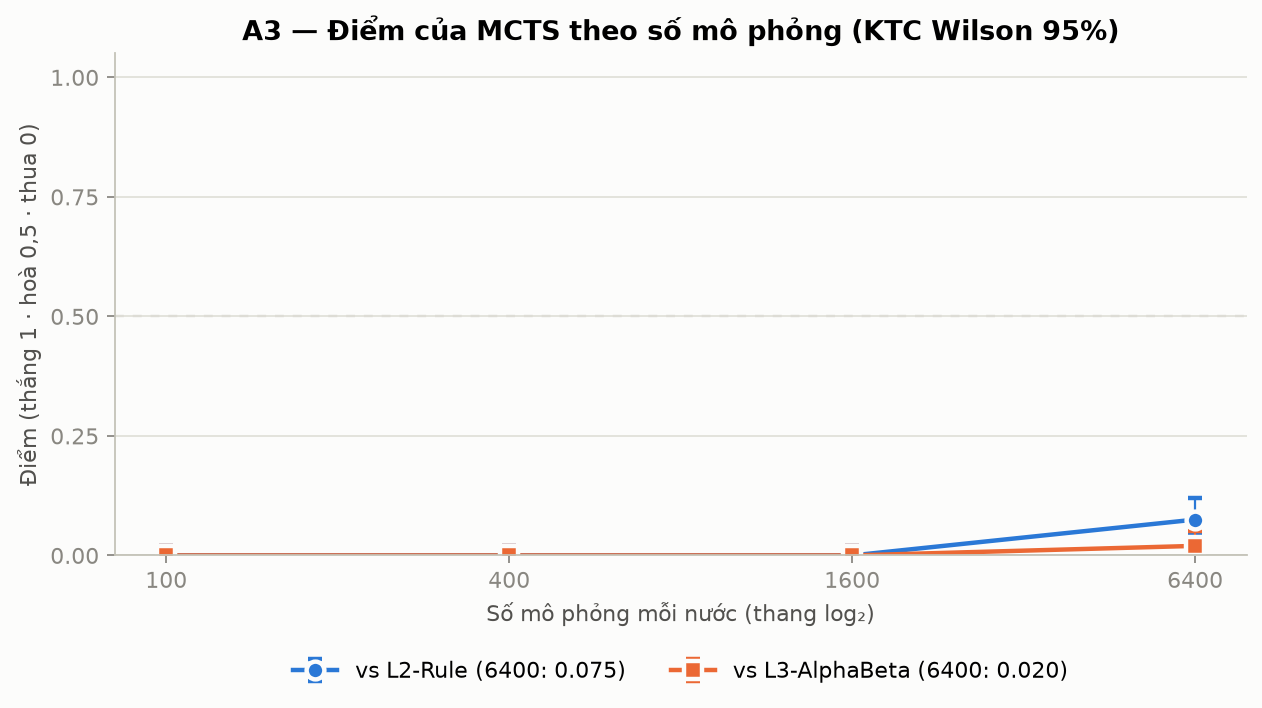
\includegraphics[width=.72\textwidth]{thuc-nghiem/a3_diem_theo_sims.png}
  \caption{A3: điểm của MCTS theo $\log_2$ số mô phỏng, có khoảng tin cậy Wilson 95\%.}
\end{figure}

\subsection{A4: kiểu rollout của MCTS}
\textbf{Thiết lập.} Giữ 800 mô phỏng, đổi rollout giữa \texttt{random} và \texttt{light}, cùng đối thủ và cùng số ván như A3 (800 ván trong 9 phút). Log: \texttt{runs/tournament/a4\_rollout/20261114-234556}.

\begin{table}[h]
  \centering\small
  \begin{tabular}{@{}lrrrr@{}}
    \toprule
    Rollout & Điểm vs cấp 2 / cấp 3 & TB (ms/nước) & p95 (ms) & mp/s \\
    \midrule
    \texttt{random} & 0,000 / 0,000 & 147,2 & 177,8 & \num{5435} \\
    \texttt{light} & 0,000 / 0,000 & 551,7 & 745,8 & \num{1450} \\
    \bottomrule
  \end{tabular}
  \caption{A4: so sánh hai kiểu rollout ở 800 mô phỏng, $n=200$ ván mỗi ô.}
\end{table}

\subsection{Phân tích A3 và A4}
Với 100, 400 và 1600 mô phỏng, MCTS thua toàn bộ 400 ván. Chỉ ở 6400 mô phỏng mới có ván thắng: bước tăng cuối đạt $+0{,}075$ trước cấp 2 với hai khoảng tin cậy tách rời, còn trước cấp 3 là $+0{,}020$ và hai khoảng chồng lấn. Thời gian mỗi nước tăng gần tuyến tính theo số mô phỏng. Ở A4, cả hai kiểu rollout đều thua toàn bộ ván, nên điểm số \emph{không phân biệt được} hai kiểu; chỉ chi phí khác rõ: rollout nhẹ chậm hơn khoảng $3{,}7$ lần.

Nhóm đã kiểm tra rằng kết quả không do lỗi cài đặt: MCTS 400 mô phỏng với rollout nhẹ đấu 10 ván với Random, đổi màu, thắng 10/10. Nguyên nhân thực sự là thiếu nhìn xa về chiến thuật. Ví dụ MCTS không chặn một ba hở trên đường chéo, đối thủ tiếp tục thành tứ hở và thắng. Muốn thấy tình huống đó cần cây sâu khoảng 4 ply, trong khi 800 mô phỏng chia cho khoảng 40 nước ở gốc chỉ cho mỗi nước chừng 20 lượt thăm. Rollout nhẹ chỉ thắng hoặc chặn \emph{ngay lập tức} nên không bù được chỗ này, và cả cấp 2 lẫn cấp 3 đều có sẵn luật chiến thuật để khai thác điểm yếu đó. Hệ quả: ván kết thúc rất sớm, trung bình khoảng 10 đến 12 nước.

Kết luận hiện tại chỉ ở mức thực nghiệm: tăng số mô phỏng chỉ có tác dụng ở mức rất cao, và A4 chưa đủ sức phân biệt hai rollout. Để trả lời RQ1 đầy đủ cần thêm đối thủ yếu hơn để điểm không dồn về 0, và đối chiếu với chế độ A (cùng thời gian mỗi nước). Thí nghiệm A8 (MCTS có và không có \texttt{root\_tactics}) nhằm kiểm tra trực tiếp giả thuyết thiếu chiến thuật ở gốc.

\subsection{Một cảnh báo về tính tái lập của A1, A2, A7}
Ba phép đo A1, A2 và A7 chạy ngày 29/10, trong khi tối ưu \texttt{\_threat\_info} và sắp xếp nước của \texttt{alphabeta.py} chỉ được commit và merge ngày 15/11 (commit \texttt{c7ebe18}). Trong một phép đo riêng, nhóm thấy bản chưa tối ưu chậm hơn bản tối ưu khoảng $7{,}4$ lần trên cùng bài (10 ván Alpha-Beta độ sâu 3, cùng 231 nước, 70,8 giây so với 9,5 giây) và cho cùng chuỗi nước. Vì vậy \textbf{số nút và giá trị gốc ở A1, A2, A7 vẫn đúng, nhưng các số thời gian (ms) cần đo lại} trước khi đưa vào báo cáo chính.

% ============================== 5 ==============================
\section{CẤP 5: HỌC CÓ GIÁM SÁT}

\subsection{Quy trình}
Cấp 5 gồm hai bước tách biệt: sinh dữ liệu chuyên gia, rồi huấn luyện mạng bắt chước.

\begin{figure}[h]
  \centering
  \begin{tikzpicture}[
      >=Stealth, node distance=0.55cm,
      box/.style={draw=xanhdam, fill=xanhnhat, rounded corners=2pt, align=center, minimum height=1.05cm, text width=2.7cm, font=\footnotesize},
      note/.style={font=\scriptsize\itshape, text=gray!70!black, align=center}]
    \node[box] (a) {Alpha-Beta cấp 3\\độ sâu 3, top-3};
    \node[box, right=of a] (b) {Dữ liệu chuyên gia\\trạng thái, policy, value};
    \node[box, right=of b] (c) {Huấn luyện\\\texttt{train\_sl} (GPU)};
    \node[box, right=of c] (d) {Mô hình cấp 5\\\texttt{best.pt}};
    \draw[->, line width=.8pt] (a) -- (b);
    \draw[->, line width=.8pt] (b) -- (c);
    \draw[->, line width=.8pt] (c) -- (d);
    \node[note, below=2pt of a] {\textbf{Bước 1} (CPU, đang chậm)};
    \node[note, below=2pt of c] {\textbf{Bước 2} (chưa chạy)};
  \end{tikzpicture}
  \caption{Hai bước của cấp 5. Bước 1 chạy trên CPU và là điểm nghẽn hiện tại; bước 2 chạy trên GPU.}
\end{figure}

\subsection{Sinh dữ liệu chuyên gia}
Script \texttt{gen\_expert\_data.py} cho Alpha-Beta cấp 3 tự chơi. Tại mỗi nước, \texttt{scored\_moves} trả về top-3 nước tốt nhất kèm điểm. Policy mục tiêu là softmax của ba điểm này với nhiệt độ $0{,}5$, trải trên 121 ô (ba ô khác 0, còn lại bằng 0). Nước thật được \emph{lấy mẫu} từ ba nước đó chứ không phải lúc nào cũng đi nước tốt nhất, để các ván đa dạng hơn. Mỗi ván mở đầu bằng một khai cuộc ngẫu nhiên; mỗi nước ghi một mẫu gồm trạng thái $4\times11\times11$, policy mục tiêu và kết quả ván làm value mục tiêu. Script ghi tiến độ vào \texttt{expert\_dataset\_progress.jsonl} nên dừng được và chạy tiếp được, và chạy song song bằng nhiều tiến trình. Cấu hình: độ sâu 3, top-3, nhiệt độ $0{,}5$, \num{20000} ván, 8 worker. Cấu hình còn quy định chia dữ liệu theo \emph{ván} (80/10/10) và loại trùng theo khoá chuẩn hoá qua 8 phép đối xứng; nhóm chưa kiểm tra mã hiện tại đã thực hiện đủ hai bước này chưa (\texttt{train\_sl.py} hiện chia theo thứ tự mẫu chứ không theo ván), nên đây là việc cần rà soát.

\subsection{Huấn luyện có giám sát}
Mạng \texttt{CaroResNet} gồm một lớp tích chập đầu, 6 khối residual 64 kênh, rồi hai đầu: policy (121 logit) và value (một số trong $[-1, 1]$), khoảng $0{,}48$ triệu tham số theo cấu hình. Hàm mất mát là $L = \mathrm{CE}(\pi, \pi^{\ast}) + c_v\,(v - z)^2$ với $c_v = 1$. Cấu hình huấn luyện: Adam, tốc độ học $10^{-3}$, weight decay $10^{-4}$, lô 256, tối đa 30 epoch, dừng sớm theo \texttt{val\_loss} với patience 5, tăng cường dữ liệu theo 8 đối xứng chỉ áp dụng cho tập huấn luyện (thí nghiệm A6 tắt để so sánh). Cấu hình yêu cầu đánh giá với các tác tử cấp 1, 2 và 3 sau mỗi epoch; mã hiện tại mới in thông báo chứ chưa thực sự đấu (mục~\ref{sec:rui-ro}).

% ============================== 6 ==============================
\section{CẤP 6: REINFORCE CÓ BASELINE}
Phần cài đặt nằm ở commit \texttt{af8312f} trên nhánh \texttt{feat/l6-reinforce}, chưa merge vào \texttt{main}.

\subsection{Thuật toán}
Mỗi vòng lặp chơi song song \texttt{batch\_games} $= 128$ ván, suy luận theo lô cho mọi ván đang chơi, rồi cập nhật tham số một bước. Mỗi ván bắt đầu bằng 2 nước khai cuộc ngẫu nhiên trong vùng $5\times5$ giữa bàn để tránh ván giống nhau, và bên học xen kẽ giữa X và O. Gọi $z \in \{+1, 0, -1\}$ là kết quả ván theo góc nhìn của bên vừa đi (thưởng chỉ có ở cuối ván, $\gamma = 1$) và $v(s)$ là đầu ra value head. Hàm mất mát:
\[
  L = -\,\mathbb{E}\big[(z - v(s))\log \pi(a \mid s)\big] \;+\; c_v\,\mathbb{E}\big[(v(s) - z)^2\big] \;-\; \beta\,\mathbb{E}\big[H(\pi(\cdot \mid s))\big].
\]
Lợi thế $z - v(s)$ dùng $v(s)$ làm baseline để giảm phương sai và không truyền gradient của policy ngược vào $v$, nên value head chỉ học qua số hạng sai số bình phương. Hệ số entropy $\beta$ bắt đầu từ $0{,}01$ và nhân với $0{,}999$ sau mỗi vòng để mạng bớt khám phá dần.

\subsection{Đối thủ và đánh giá}
Mỗi ván, với xác suất $0{,}5$ mạng tự chơi với bản mới nhất (cả hai bên đều được học), còn lại đấu với một checkpoint cũ trong pool (đóng băng, chỉ học nước của bên học). Pool nhận thêm một bản mỗi 5 vòng và mỗi lần đánh giá, nhằm tránh mạng chỉ thích nghi với chính nó. Cứ mỗi \num{1000} ván, mạng được đóng băng và đấu 100 ván đổi màu (chọn nước tốt nhất, không tìm kiếm) với cấp 2 và cấp 3, ghi điểm kèm khoảng Wilson vào \texttt{metrics.jsonl} để vẽ learning curve; hai checkpoint \texttt{last.pt} và \texttt{best.pt} được lưu.

\subsection{Các điểm kỹ thuật}
Đặc trưng đầu vào tính bằng numpy cho nhanh nhưng được kiểm thử bằng số khớp với \texttt{board\_to\_tensor}. Tham số \texttt{update\_chunk} $= 1024$ chia các mẫu của một vòng thành lô con và cộng dồn gradient để vừa bộ nhớ GPU, với trung bình tính theo số mẫu chứ không theo lô con. Gradient được cắt chuẩn tại $1{,}0$.

\begin{table}[h]
  \centering\small
  \begin{tabular}{@{}lr@{\qquad}lr@{}}
    \toprule
    Tham số & Giá trị & Tham số & Giá trị \\
    \midrule
    Số ván huấn luyện & \num{50000} & Tốc độ học (Adam) & $2\cdot10^{-4}$ \\
    Ván mỗi vòng & 128 & $\beta$ ban đầu / hệ số giảm & $0{,}01$ / $0{,}999$ \\
    Nhiệt độ lấy mẫu & $1{,}0$ & Cắt chuẩn gradient & $1{,}0$ \\
    Khởi tạo & \texttt{model:l5} & Đánh giá mỗi & \num{1000} ván \\
    \bottomrule
  \end{tabular}
  \caption{Cấu hình huấn luyện cấp 6. Thí nghiệm A5b dùng \texttt{train.init=random} để so với khởi tạo từ cấp 5.}
\end{table}

\subsection{Kiểm thử}
\texttt{tests/test\_train\_pg.py} có 7 kiểm thử: đặc trưng nhanh khớp \texttt{board\_to\_tensor} trên các thế cờ ngẫu nhiên, mặt nạ nước hợp lệ, một bước cập nhật làm thay đổi trọng số và trả đủ các loại loss, và một lần huấn luyện nhỏ chạy hết trên CPU (có đánh giá, ghi metrics, lưu checkpoint). Nhóm chưa chạy huấn luyện cấp 6 ở quy mô thật nên chưa có learning curve.

% ============================== 7 ==============================
\section{ĐO ĐẠC THỜI GIAN SINH DỮ LIỆU CẤP 5}\label{sec:thoigian}

\subsection{Phương pháp đo}
Máy đo: Intel Core i7-11800H (8 lõi vật lý, 16 luồng), GPU RTX A2000, RAM 15 GB. Mọi số liệu dưới đây do nhóm đo trực tiếp bằng đúng đường chạy mà script sinh dữ liệu dùng, thông qua mã đo tạm không nằm trong mã nguồn chính.
\begin{gon}
  \item \textbf{Chạy 5 phút:} chạy script với cấu hình thật, 8 worker, dừng sau đúng 300 giây rồi đếm số ván hoàn thành trong file tiến độ.
  \item \textbf{So sánh hai đường chạy:} cho tác tử tự chơi 3 ván ở độ sâu 3 bằng \texttt{select\_action} và bằng \texttt{scored\_moves}, tính thời gian trung bình mỗi nước.
  \item \textbf{Thử cắt tỉa:} lấy 40 thế cờ từ 6 ván tự chơi, chạy ba phương án trên cùng 40 thế và so thời gian cùng tập (nước, điểm) top-3.
\end{gon}

\subsection{Kết quả}
\begin{table}[h]
  \centering\small
  \begin{tabular}{@{}lr@{}}
    \toprule
    Phép đo & Kết quả \\
    \midrule
    Chạy thật 5 phút, 8 worker & 141 ván, \num{3358} mẫu \\
    Tốc độ & $\approx 0{,}47$ ván/giây ($\approx 28$ ván/phút) \\
    Mẫu trung bình mỗi ván & $\approx 24$ \\
    Ước tính cho \num{20000} ván (bản hiện tại) & $\approx 11{,}8$ giờ \\
    \texttt{select\_action}, mỗi nước & $0{,}040$ giây \\
    \texttt{scored\_moves}, mỗi nước & $0{,}452$ giây \\
    \bottomrule
  \end{tabular}
  \caption{Số đo thời gian sinh dữ liệu chuyên gia trên máy của nhóm.}
\end{table}
Ước tính $11{,}8$ giờ lấy từ $20000 / 0{,}47 \approx 42\,500$ giây. Một lần đo ngắn hơn trước đó (16 ván trên 16 worker) cho ước tính cao hơn, khoảng 15 giờ, vì thời gian bị kéo dài bởi ván chậm nhất trong nhóm; nhóm lấy số đo 5 phút làm chuẩn. Đặt 16 worker không nhanh hơn 8 là bao do máy chỉ có 8 lõi vật lý: thời gian CPU tổng cộng 387 giây trong 46 giây thực, tức song song hoá thực tế chỉ khoảng $8{,}4$ lần.

\subsection{Nguyên nhân chậm}
Hàm \texttt{scored\_moves} duyệt mọi nước ứng viên ở gốc (vùng bán kính 2 quanh các quân, thường vài chục nước) và search từng nước với cửa sổ $(-\infty, +\infty)$. Vì cửa sổ luôn mở rộng, điểm của những nước đã tìm không được dùng để cắt tỉa các nước sau, trong khi dữ liệu chỉ cần top-3. So với \texttt{select\_action} (chỉ tìm một nước, có cắt tỉa trọn vẹn), chi phí mỗi nước cao hơn khoảng 11 lần. Ngoài ra, Alpha-Beta cài bằng Python tuần tự trên bitboard nên GPU không giúp được bước này: cắt tỉa phụ thuộc kết quả nhánh trước, không phải phép tính song song đồng nhất. Muốn rút ngắn cần giảm công việc tìm kiếm hoặc tăng số lõi CPU.

\textbf{Đính chính.} Một ước tính trước đó (khoảng 40 phút) đo trên \texttt{select\_action} chứ không phải \texttt{scored\_moves}, nên thấp hơn thực tế khoảng 25 lần mỗi ván. Số liệu trong báo cáo này đo trên đúng đường chạy mà script sinh dữ liệu dùng.

\subsection{Thử nghiệm cắt tỉa ở gốc}
Ý tưởng: sau khi đã tìm được ít nhất $k = 3$ nước, gọi $\theta$ là điểm tốt thứ $k$ hiện có. Với mỗi nước còn lại, chỉ cần biết điểm của nước đó \emph{có vượt $\theta$ hay không}. Vì điểm là số nguyên và search con trả điểm theo góc nhìn đối thủ, ta gọi search con với cửa sổ $(-\infty,\; -\theta + 1)$. Nếu nước không vượt $\theta$ thì nhánh bị cắt sớm, điểm trả về chỉ là một cận và nước đó nằm ngoài top-3 nên không dùng. Nước vượt $\theta$ vẫn được tính chính xác và $\theta$ được cập nhật. Ba nước đầu cửa sổ vẫn mở hoàn toàn.

\begin{table}[h]
  \centering\small
  \begin{tabular}{@{}lrrr@{}}
    \toprule
    Phương án & Thời gian (giây) & Nhanh hơn & Top-3 trùng bản cũ \\
    \midrule
    Bản hiện tại & $5{,}9$ & $1\times$ & (chuẩn) \\
    Cắt tỉa ở gốc & $1{,}7$ & $3{,}4\times$ & 40/40 \\
    Cắt tỉa và sắp xếp nước ở gốc & $0{,}8$ & $7{,}3\times$ & 31/40 \\
    \bottomrule
  \end{tabular}
  \caption{Kết quả thử nghiệm sơ bộ trên 40 thế cờ (thời gian chạy toàn bộ 40 thế).}
\end{table}
Cắt tỉa ở gốc giữ nguyên top-3 trên toàn bộ 40 thế nên có thể áp dụng; suy ra thời gian sinh \num{20000} ván còn khoảng $11{,}8 / 3{,}4 \approx 3{,}5$ giờ. Bản có sắp xếp nước (xếp trước các nước có điểm nông cao) nhanh hơn nhưng lệch 9/40 thế. Nhóm chưa biết đó là hoà điểm ở hạng ba (hai nước cùng điểm nên tập top-3 khác nhau mà vẫn đúng) hay là lỗi thật, nên chưa dùng bản này và sẽ điều tra riêng. Hạn chế của thử nghiệm: mẫu nhỏ (40 thế, 6 ván) và các thế cách nhau một nước, nên mức tăng tốc thực tế có thể khác ở đầu và cuối ván.

\subsection{Các phương án khác}
\begin{itemize}
  \item \textbf{Thuê máy nhiều lõi.} Các ván độc lập nên tốc độ tăng gần tuyến tính theo số lõi vật lý; dịch vụ như VNG Cloud, FPT Cloud, Viettel Cloud, Bizfly Cloud trong nước, hoặc Hetzner, Vultr, DigitalOcean ở nước ngoài. Các dịch vụ miễn phí như Kaggle hay Colab chỉ cấp ít lõi CPU nên không giải quyết được vấn đề này. Số liệu giá và cấu hình cần được kiểm tra lại trước khi quyết định.
  \item \textbf{Giảm số ván} xuống khoảng \num{8000}, cho khoảng 190 nghìn mẫu. Cách này đổi dữ liệu lấy thời gian và cần đối chiếu với báo cáo chính.
  \item \textbf{Giảm độ sâu chuyên gia} từ 3 xuống 2: nhanh hơn nhiều nhưng chuyên gia yếu đi và lệch so với mô tả trong báo cáo, nhóm không khuyến nghị.
\end{itemize}

% ============================== 8 ==============================
\section{RỦI RO VÀ VẤN ĐỀ TỒN TẠI}\label{sec:rui-ro}
\begin{enumerate}
  \item \textbf{Tràn bộ nhớ khi huấn luyện cấp 5.} \texttt{train\_sl.py} nạp toàn bộ file JSON vào RAM dưới dạng list Python. \num{20000} ván cho khoảng $4{,}8\cdot10^5$ mẫu; mỗi mẫu gồm 484 giá trị trạng thái và 121 giá trị policy, nên ước tính vượt 9 GB khi nạp, trong khi máy chỉ còn khoảng 6 GB trống. Cách xử lý đề xuất: lưu dữ liệu dạng mảng nhị phân (\texttt{.npz}) và nạp bằng \texttt{numpy} (\texttt{float32}, khoảng $1{,}2$ GB, hoặc nhỏ hơn nếu nén).
  \item \textbf{Hạn chế của \texttt{train\_sl.py}.} Không nhận override từ dòng lệnh (A6 cần \texttt{data.augment\_x8=false}), chưa đánh giá với cấp 1 đến 3 theo \texttt{eval\_vs}, chưa ghi log qua \texttt{Run} như cấp 6, và sẽ huấn luyện trên dữ liệu giả nếu thiếu file dữ liệu mà không báo lỗi. \texttt{gen\_expert\_data.py} cũng không nhận override.
  \item \textbf{Mã dùng chung.} Cắt tỉa ở gốc cần sửa \texttt{alphabeta.py}, mã dùng chung với cấp 3, nên phải có kiểm thử so top-3 với bản cũ để không ảnh hưởng các thí nghiệm A1 đến A4.
  \item \textbf{Tính tái lập.} A1, A3, A4 và A7 chạy trên working tree chưa commit (\texttt{dirty: true} trong \texttt{meta.json}); các số thời gian của A1, A2, A7 cần đo lại (mục~\ref{sec:thucnghiem}); A2 thiếu độ sâu đạt được. Nên chạy lại từ một commit sạch trước khi đưa số vào báo cáo chính.
  \item \textbf{Điểm số dồn về 0.} Ở A3 và A4, MCTS thua gần như mọi ván nên điểm không phân biệt được các cấu hình; cần đối thủ yếu hơn hoặc chế độ A.
  \item \textbf{Khác biệt tài liệu.} Chú thích kênh đầu vào trong \texttt{resnet\_small.yaml} không hoàn toàn khớp cách mã hoá thực tế trong \texttt{board\_to\_tensor}; cần đối chiếu và sửa chú thích để báo cáo mô tả đúng.
  \item \textbf{Thời gian huấn luyện cấp 6 và 8.} Chưa đo tốc độ tự chơi trên GPU, nên chưa biết \num{50000} ván tốn bao lâu; cần chạy thử ngắn trước khi chạy thật.
\end{enumerate}

% ============================== 9 ==============================
\section{KẾ HOẠCH TIẾP THEO}
\begin{table}[h]
  \centering\small
  \begin{tabularx}{\textwidth}{@{}c X X@{}}
    \toprule
    Bước & Công việc & Tiêu chí hoàn thành \\
    \midrule
    1 & Đưa cắt tỉa ở gốc vào \texttt{scored\_moves}, thêm kiểm thử & Top-3 trùng bản cũ trên tập thế cờ ngẫu nhiên; kiểm thử đạt \\
    2 & Chạy lại phép đo 5 phút, rồi sinh đủ \num{20000} ván ở nền (8 worker) & Số ván mỗi 5 phút tăng rõ so với 141; có \texttt{expert\_dataset} đủ ván \\
    3 & Sửa \texttt{train\_sl.py}: dữ liệu nhị phân, override, đánh giá cấp 1 đến 3, log qua \texttt{Run} & Chạy hết với dữ liệu thật mà không tràn RAM \\
    4 & Huấn luyện cấp 5 trên GPU & Có checkpoint và đường cong \texttt{val\_loss}; điểm đấu với cấp 1 đến 3 \\
    5 & Dùng cấp 5 khởi tạo cho cấp 6, chạy thí nghiệm A5b & Learning curve cấp 6 so với khởi tạo ngẫu nhiên \\
    6 & Điều tra chênh lệch 9/40 của bản có sắp xếp nước & Biết rõ là hoà điểm hay lỗi; nếu vô hại thì áp dụng \\
    7 & Đo lại A1, A2, A7 từ commit sạch; ghi độ sâu cho A2 & Số liệu thời gian cập nhật, có \texttt{dirty: false} \\
    8 & Chạy A8 và bổ sung đối thủ yếu cho A3, A4 & Điểm không còn dồn về 0, phân biệt được rollout \\
    9 & Cấp 7 PUCT và cấp 8 AlphaZero, thí nghiệm A5, A6, E3 & Có mô hình và kết quả cho RQ2 \\
    10 & Giải đấu chính ở hai chế độ A và B, phân tích và viết báo cáo & Ma trận đối đầu, Elo, trả lời RQ1 đến RQ4 \\
    \bottomrule
  \end{tabularx}
  \caption{Kế hoạch công việc.}
\end{table}

\subsection{Các quyết định cần thống nhất}
\begin{itemize}
  \item Chạy đủ \num{20000} ván hay giảm xuống khoảng \num{8000} nếu sau tối ưu vẫn quá lâu.
  \item Có thuê máy nhiều lõi để sinh dữ liệu hay chạy qua đêm trên máy hiện có.
  \item Thời điểm merge \texttt{feat/l6-reinforce} vào \texttt{main} và tạo pull request.
  \item Có cần chạy lại các giải đấu A3 và A4 với đối thủ yếu hơn trước khi viết phần thảo luận.
\end{itemize}

\end{document}
